Visualizando la figura \ref{fig:time} se aprecia como el algoritmo clásico es más inestable en cuanto al tiempo que tarda en lograr la factorización del número
a comparación del algoritmo de Shor el cual mantiene tiempos semejenates durante cada repetición, esto puede ser debido a que el algoritmo de Shor maneja una serie 
de pasos como el calculo del periodo de a función a\textsuperscript{x}mod N.\\
Lo más facil de ver es el tiempo medio que tarda cada algoritmo en obtener el resultado, esto es mostrado en la tabla \ref{tabla:resultados}, en este caso el algoritmo de Shor
ejecutado en una computadora cuántica es el más rápido en promedio, las diferencias entre al algoritmo de Shor ejecutado de en una computadora clásica y ejecutado en una computadora
cuántica son debido a que en la clásica se tiene que simular cada estado cuántico, en cambio en la cuántica este estado es preparado y medido experimentalmente.\\\\

Un problema que nos encontramos al momento de ejecutar los códigos del algoritmo de Shor (código \ref{cod:shorquanrum}) dentro del sistema de \href{https://quantum-computing.ibm.com/}{\textit{IBM Q Experience}} fue el número que podiamos introducir en el código, ya que
el dispositivo que ellos tienen es de 5 qbits, por lo que el número más grande que se puede introducir al día de hoy es el 31, es por ello que aun no se puede comprobar experimentalmente
la eficiencia de los algoritmos para números muy grandes, al menos de manera al publico en general pero con estos resultados podemos observar una mayor eficiencia y estabilidad en los calculos que se 
realicen dentro de una computadora cuántica siguiendo conceptos y principios cuánticos.
\begin{figure}[H]
    \begin{subfigure}{0.19\linewidth}
        \centering
        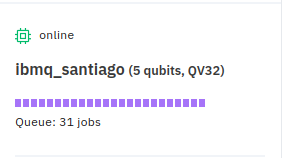
\includegraphics[scale=0.35]{images/santiago.png}
    \end{subfigure}
    \begin{subfigure}{0.19\linewidth}
        \centering
        
\includegraphics[scale=0.35]{images/athrens.png}
    \end{subfigure}
    \begin{subfigure}{0.19\linewidth}
        \centering
        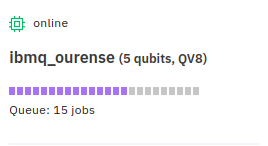
\includegraphics[scale=0.35]{images/ourense.png}
    \end{subfigure}
    \begin{subfigure}{0.19\linewidth}
        \centering
        
\includegraphics[scale=0.35]{images/valencia.png}
    \end{subfigure}
    \begin{subfigure}{0.19\linewidth}
        \centering
        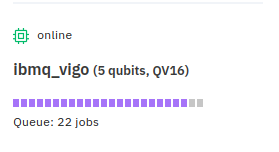
\includegraphics[scale=0.35]{images/vigo.png}
    \end{subfigure}
    \caption{Lista de dispositivos disponibles al público desde \href{https://quantum-computing.ibm.com/}{\textit{IBM Q Experience}}}
\end{figure}